\subsection{Investigation}
This phase of the project may be considered as the most time-consuming and longest in development, as it does not contain any end goals that can be achieved by simple code implementation.
Throughout development, it reentered several phases of rethinking and rediscovering the process of very particular approaches.\\
There is no end to this section as it gets updated with every discovery, observation and result.
It suffered from inevitable changes, and, as it provided some exciting discoveries.
Finally, it will be summarised in a subsection by each hardware and software component.
\subsubsection{$360\circ$ camera}
One of the parts for recreating the surrounding environment is a 360-degree camera on Figure~\ref{fig:camera} on the right. 
In this case, the Kodak PIXPRO SP360 became the only available option.
However, despite the product cost, it was discovered that it is suited more for casual or touristic usage, rather than a severe component for upfront research.
It allows setting the recording stream to 60 frames per second (fps) with a 4k resolution, which allows for achieving high accuracy on a resulting image.
However, such video stream scale brings specific software difficulties as it requires preprocessing due to the memory size of the output.
PIXPRO also contains a useful application, allowing the establishment of a connection between the computer and the camera using either WiFi or NFC, which completely resolves the issue with storage.
Resulted video streams allow investigation of a full surrounding range with a decent elevation angle.
To use the device for other applications \footnote{except the official one}, it provides an easily accessible link, within a local IP address.
\begin{equation*}
 http://172.16.0.254:9176/
\end{equation*}
\begin{wrapfigure}{r}{0.35\textwidth}
    \centering
    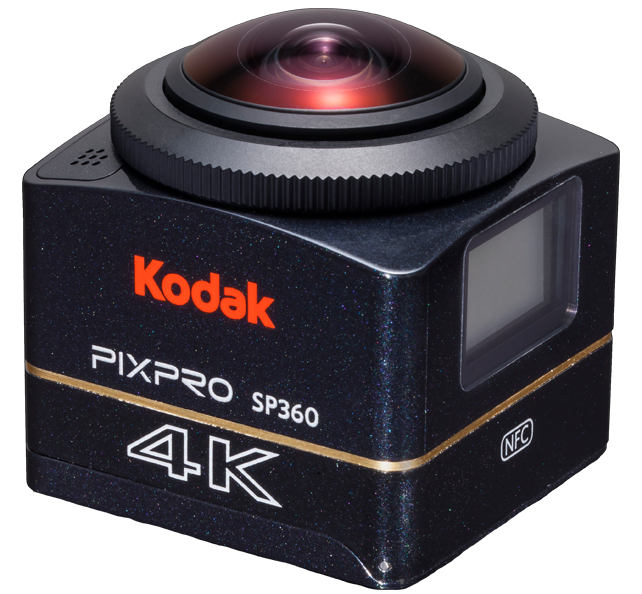
\includegraphics[width=0.30\textwidth]{project/images/camera.png}
    \caption{Kodak SP360}
    \label{fig:camera}
\end{wrapfigure}
Despite the high quality and good enough response speed, the drawback which the project met, is the format of the recording.
It talks about video output by format, which produced a hemisphere output. 
The problem with this stream is the actual usability.\\[1pc]
The Pixpro application setting does not allow the modification of the data stream upon recording.
The Unity Game engine supports dealing with a spherical or cubic texture. 
By providing it with only half of the image, the sphere got corrupted, and reconstructed video could barely consider as appropriate.\\[1pc]
An FFmpeg tool played its role very well in resolving this matter. 
However, by using an extra layer of configuration, video stream response gets slower, which requires sacrificing the quality of video in general. \\
The problem has resolved itself with some effort and video manipulation, but that was not the only one.\\[1pc]
The second issue is more problematic than simple software manipulation.
The PIXPRO application did not provide any means for changing settings. 
It served only as a trigger to start the recording process.\footnote{This particular issue was utterly ignored since the previous developer faced a similar problem.}
The best resolution to that is to replace the camera completely.
Some Raspberry Pi kits contain external cameras with a 360-degree view.
Maybe they can serve as a proper replacement.\\[1pc]
Originally, the camera was meant to serve both as a video stream and as a communication host between Unity, Tank and any other necessary components.
It turns out that additional devices \textbf{cannot} communicate with each other, over Camera WiFi hotspot. \\
The whole IP range is located within 172.16.1.* range, starting from 1 and 255(excluding 254). Such a weird configuration exists due to the way not to interfere with the actual video stream IP on location 254.
All credits to this discovery belong to \textit{nmap} network tool.
For only local usage, this tool was considered legitimate as there were no other alternatives.\\
The triggered issue, which required a total camera replacement, will be discussed later in Raspberry Pi subsection~\ref{subsec:RPI}.\\[1pc]
Finally, the delay between recording and actual reconstruction within a game is a separate matter to resolve.
The delay turned out to be significant since the video stream had to be modified and reapplied as textures following UDP protocol, instead of https, which will be discussed in Unity subsection~\ref{subsubsec:Unity}.
The previous argument ends up to be as another reason to replace this particular hardware with something more useful.
\subsubsection{Object Detection \& Machine Learning Nets}
The original idea of using a simple OpenCV library has proven to be quite useful in other similar kinds of projects, but not for this one, which takes much processing to care first.
It also showed good results after running some simple tests with a web camera to detect a specific object.
OpenCV has proven to be very good, in particular, to recognise the yellow colour as potential targets.
Initially, they were meant to look like small pong balls.
However, having something more powerful and experience in Machine Learning had to play itself more efficiently. \\[1pc]
During the general university study, outside of research time, there were several tasks in hand that required a certain degree of machine learning usage, TensorFlow in particular.
With the help of researchers and Lecturers, knowledge gained from their expertise becomes a significant contribution towards building a new efficient Neural Network to recognise tanks in the 360-degree image.
It is a good thing that through serving through the World Web, there were several libraries that provided a good example and API to use TensorFlow inside Unity with C\# Language.
However, all similar projects described earlier used only the CPU level to perform calculations, which does not give the best result of processing.
Luckily, Unity is aimed to use Computer Graphics, which means the next stage of learning with use NVIDIA CUDA libraries.
So far, all detections performed well on a Linux environment, which gave higher results than Windows, but those details and how CUDA with GPU may enhance this process are meant to be investigated by other researchers.
\subsubsection{Unity Game Engine} \label{subsubsec:Unity}
\begin{wrapfigure}{r}{0.3\textwidth}
    \centering
    
\includegraphics[width=0.25\textwidth]{project/images/Unity-Logo.png}
\end{wrapfigure}
Unity is an environment based on Game Engine, which is occasionally used for simulations and testing in some companies.
As a foundation and first-hand experience, the VRES project of Kitchen Assistant (EvKA) served as a starting point.
It was also meant to be deployed in Virtual Reality (VR) with the help of some gear.
Using similar techniques may simplify the overall integration. \\[1pc]
Most of the video games implemented so far require the usage of the keyboard, mouse, joystick or similar tools.
All of them, most of the time, required the usage of hands and fingers.
VR with different hand gear allows people to perform more actions, including some physical work.
Unity in this project will be the base, where all discoveries will come up as one end-up product.
All other details of how it turned out with implementation are discussed further down.
\subsubsection{VR Gear Set}
This section is the least investigated part, even if considered as the main topic of the project.
However, the reason behind such a lack of attempts is the final goal.
HTC Vive designed for smooth integration with Unity, using SteamVR as a base for development.
Their usage, limitations and type of suitable device will be acknowledged later.
\subsubsection{Raspberry Pi} \label{subsec:RPI}
\begin{wrapfigure}{r}{0.45\textwidth}
	\begin{center}
		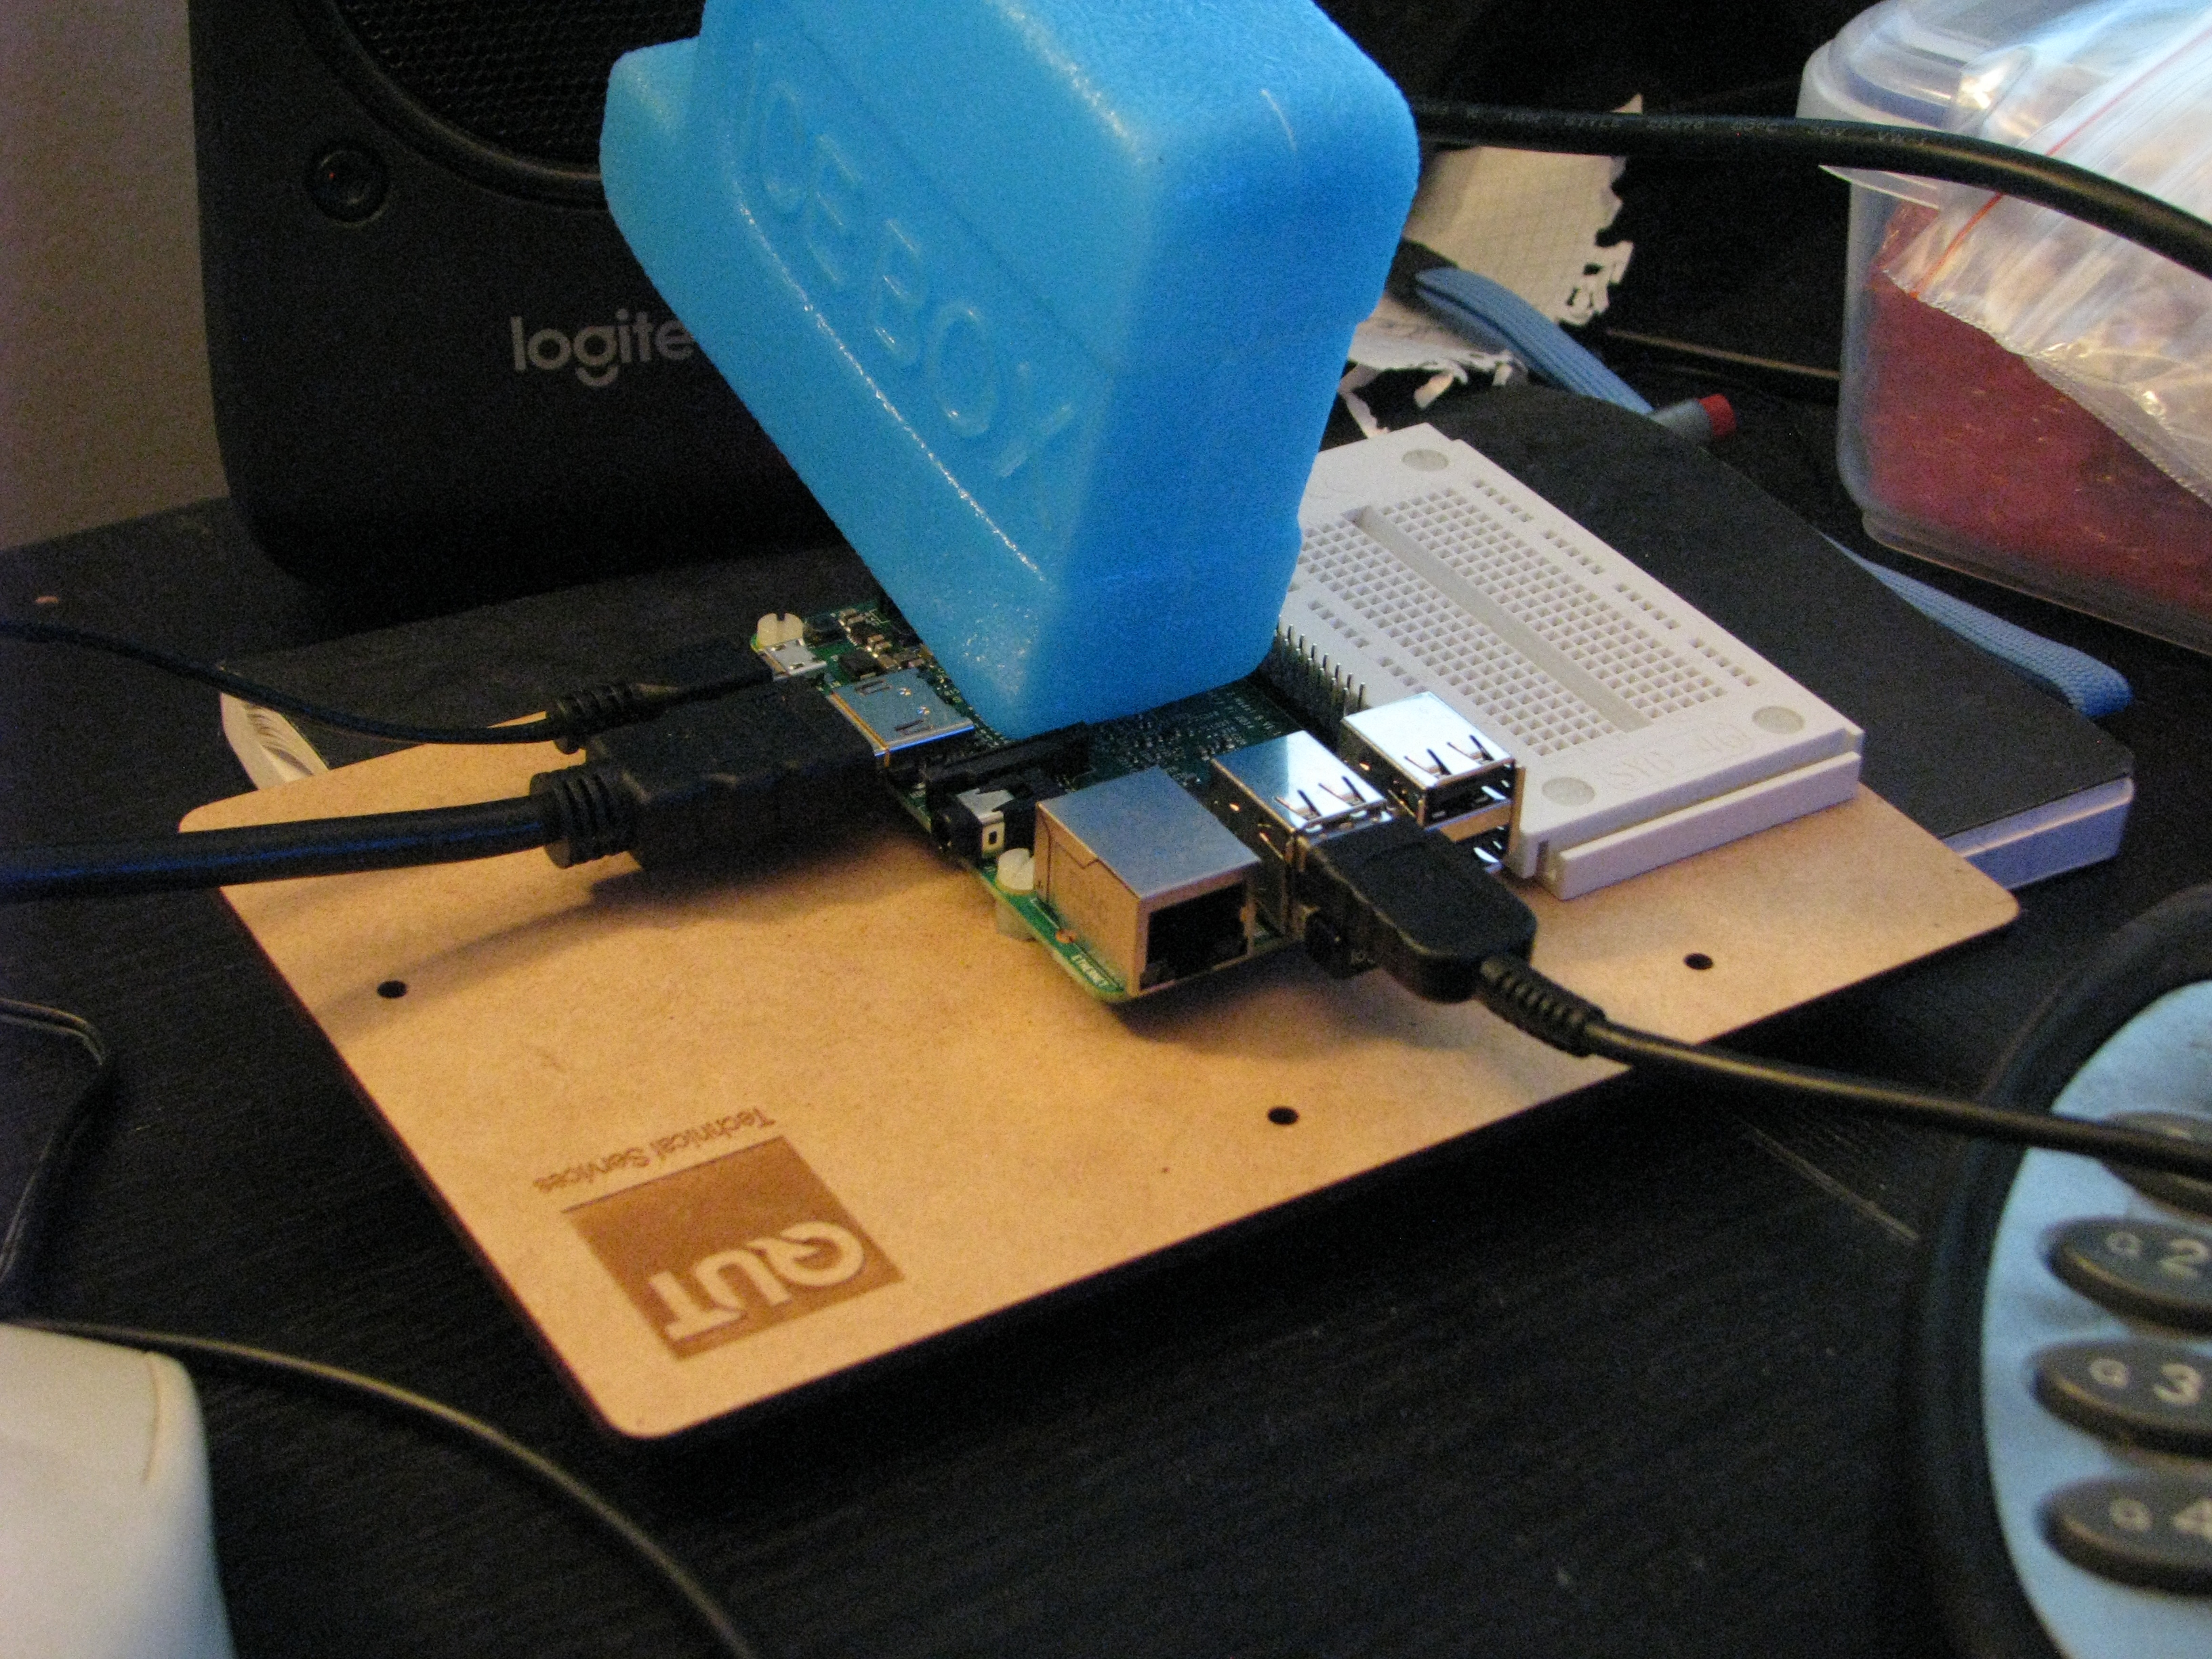
\includegraphics[width=0.35\textwidth]{project/images/IMG_1194.JPG}
	\end{center}
	\caption{Raspberry Pi cooling way}
	\label{fig:RPI}
\end{wrapfigure}
Another addition to the project and overall learning, in general, is an introduction to a new component - the controller of the tank itself. 
As a reminder, the current project builds on top of someone else's work, who constructed an actual voice-controlled tank. 
The way to send commands and drive this toy was performed using Raspberry Pi V3.
This particular version supports Wireless Communication.
R-Pi can establish a connection to a predefined WiFi hotspot and establish remote communication over either SSH or VNC. 
The Unity project will connect with Tank control over SPB, which allows mirroring all activities performed in Unity with the actual toy.
The concept of communication, package exchange or message way is used with socket communication.
By opening a socket server on Raspberry Pi through an IP address and port, Unity connects to the controller as a client and starts exchanging messages.
Through that talk, Tank will know what action is required to perform.
C\# and Python, the best message exchange package is ZMQ, after several hours of trials with different Libraries.
It is much simpler and more flexible than an ordinary socket.
The drawback of using R-Pi is the cooling system.
This particular model had to fan in the first place, that is why cooling was performed with whatever means possible, Figure~\ref{fig:RPI}.\\
Finally, Raspberry Pi contains a small circuit output - General Practice Input/Output (GPIO) pins.
They will be used to create an elementary testing circuit with LEDs on a breadboard, presented in the same Figure next to the controller.